\documentclass{beamer}

\usepackage{graphicx}
\usepackage{default}
\usepackage{amsmath}

\graphicspath{{images/}}

\title{Singular Value Decomposition (SVD)}
\author{Felipe de A. Mello Pereira, Guilherme G. Schardong, William Paulo Ducca Fernandes}

\begin{document}

\begin{frame}
  \maketitle
\end{frame}

\begin{frame}{Sum\'ario}
  \tableofcontents
\end{frame}

\section{Exerc\'icio 3.27}
\begin{frame}{Exerc\'icio 3.27 - Resultados num\'ericos}
  \begin{table}[]
    \centering
    \caption{Resultados num\'ericos da reconstru\c{c}\~{a}o usando 5\%, 10\%, 25\% e 50\% dos valores singulares.}
    \begin{tabular}{l|rrrrr}
      & \textbf{\begin{tabular}[c]{@{}r@{}}Norma\\ Original\end{tabular}} & \textbf{5\%} & \textbf{10\%} & \textbf{25\%} & \textbf{50\%} \\ \hline
      \textbf{Canal R} & 95630.79                                                          & 99.65\%      & 99.87\%       & 99.98\%       & 100\%         \\
      \textbf{Canal G} & 57488.22                                                          & 98.45\%      & 99.35\%       & 99.88\%       & 99.98\%       \\
      \textbf{Canal B} & 56717.18                                                          & 98.96\%      & 99.47\%       & 99.84\%       & 99.97\%      
    \end{tabular}
  \end{table}
\end{frame}

\begin{frame}{Exerc\'icio 3.27 - Resultados Visuais}
  \begin{figure}
    \centering
    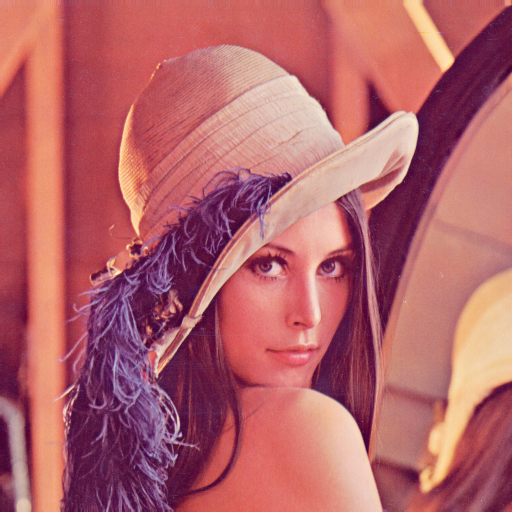
\includegraphics[width=0.65\columnwidth]{Lenna.png}
    \caption{Imagem original.}
  \end{figure}
\end{frame}

\begin{frame}{Exerc\'icio 3.27 - Resultados Visuais}
  \begin{figure}
    \centering
    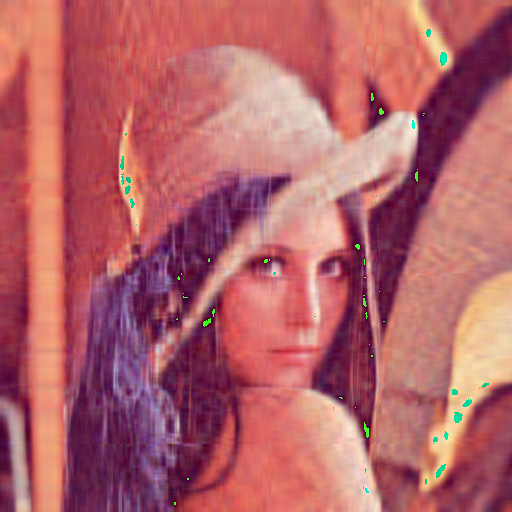
\includegraphics[width=0.65\columnwidth]{Lenna_25.png}
    \caption{Mantendo 5\% dos valores singulares.}
  \end{figure}
\end{frame}

\begin{frame}{Exerc\'icio 3.27 - Resultados Visuais}
  \begin{figure}
    \centering
    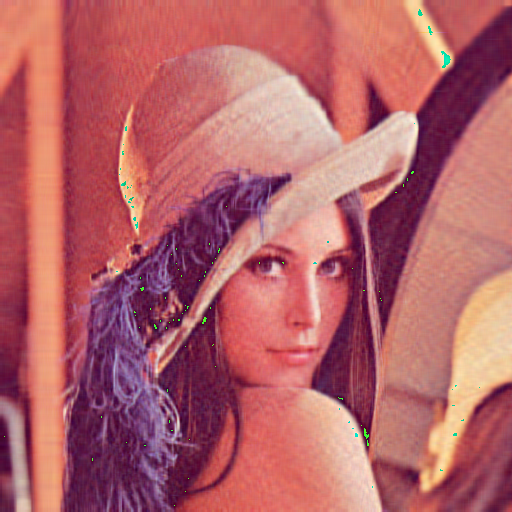
\includegraphics[width=0.65\columnwidth]{Lenna_51.png}
    \caption{Mantendo 10\% dos valores singulares.}
  \end{figure}
\end{frame}

\begin{frame}{Exerc\'icio 3.27 - Resultados Visuais}
  \begin{figure}
    \centering
    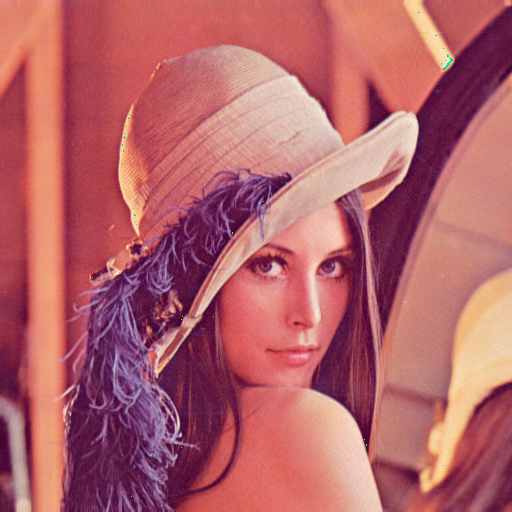
\includegraphics[width=0.65\columnwidth]{Lenna_128.png}
    \caption{Mantendo 20\% dos valores singulares.}
  \end{figure}
\end{frame}

\begin{frame}{Exerc\'icio 3.27 - Resultados Visuais}
  \begin{figure}
    \centering
    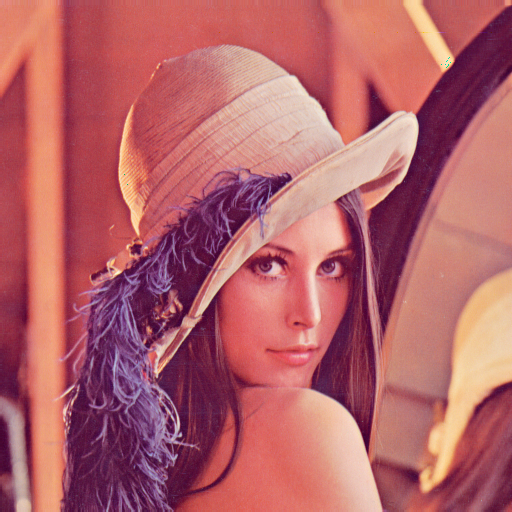
\includegraphics[width=0.65\columnwidth]{Lenna_256.png}
    \caption{Mantendo 50\% dos valores singulares.}
  \end{figure}
\end{frame}

\section{Exerc\'icio 3.30}
\begin{frame}{Exerc\'icio 3.30a}
  \begin{align}
    &-\frac{1}{2n^2} \sum_{i = 1}^{n} \sum_{j = 1}^{n} d_{ij}^2 = -\frac{1}{2n^2} \sum_{i = 1}^{n} \sum_{j = 1}^{n} <x_i - x_j, x_i - x_j> = \\ \nonumber
    = &-\frac{1}{2n^2} \sum_{i = 1}^{n} \sum_{j = 1}^{n} \left( <x_i, x_i> + <x_j, x_j> - 2<x_i, x_j> \right) = \\ \nonumber
    = &-\frac{1}{2n^2} \sum_{i = 1}^{n} \left[ n <x_i, x_i> + \sum_{j = 1}^{n} <x_j, x_j> - 2 \sum_{j = 1}^{n} <x_i, x_j> \right] = \\ \nonumber
    = &-\frac{1}{2n} \sum_{i = 1}^{n} <x_i, x_i> - \frac{1}{2n} \sum_{j = 1}^{n} <x_j, x_j> + \frac{1}{n^2} \sum_{i = 1}^{n} \sum_{j = 1}^{n} <x_i, x_j> =
  \end{align}
\end{frame}

\begin{frame}{Exerc\'icio 3.30a}
  \begin{align*}
    &-\frac{1}{2n^2} \sum_{i = 1}^{n} \sum_{j = 1}^{n} d_{ij}^2 = \\ \nonumber
    = &-\frac{1}{n} \left( \sum_{i = 1}^{n} <x_i, x_i> \right) + \frac{1}{n^2} \sum_{i = 1}^{n} <x_i, \sum_{j = 1}^{n} x_j> = \\ \nonumber
    = &-\frac{1}{n} \left( \sum_{j = 1}^{n} <x_i, x_i> \right) + \frac{1}{n^2} <\sum_{i = 1}^{n} x_i, \sum_{j = 1}^{n} x_j> = \\ \nonumber
    = &-\frac{1}{n} \sum_{i = 1}^{n} <x_i, x_i> = -\frac{1}{n} \sum_{k = 1}^{n} <x_k, x_k>
  \end{align*}
\end{frame}

\begin{frame}{Exerc\'icio 3.30a}
  \begin{align}
    \frac{1}{2n} \sum_{k = 1}^{n} d_{ik}^2 &= \frac{1}{2n} \sum_{k = 1}^{n} <x_i - x_k, x_i - x_k>  \\ \nonumber
    &= \frac{1}{2n} \sum_{k = 1}^{n} \left[ <x_i, x_i> + <x_k, x_k> - 2 <x_i, x_k> \right] = \\ \nonumber
    &= \frac{1}{2n} n <x_i, x_i> + \frac{1}{2n} \sum_{k = 1}^{n} <x_k, x_k> - \frac{1}{n} \sum_{k = 1}^{n} <x_i, x_k> = \\ \nonumber
    &= \frac{1}{2} <x_i, x_i> + \frac{1}{2n} \sum_{k = 1}^{n} <x_k, x_k> - \frac{1}{n} <x_i, \sum_{k = 1}^{n} x_k> = \\ \nonumber
    &= \frac{1}{2} <x_i, x_i> + \frac{1}{2n} \sum_{k = 1}^{n} <x_k, x_k>
  \end{align}
\end{frame}

\begin{frame} {Exerc\'icio 3.30a}
  Podemos trocar $i$ com $j$, logo:
  \[
  \begin{cases} 
    \frac{1}{2n} \sum_{j=1}^{n} d_{ij}^2 = \frac{1}{2} <x_i, x_i> + \frac{1}{2n} \sum_{k = 1}^{n} <x_k, x_k>  \\
    \frac{1}{2n} \sum_{i=1}^{n} d_{ij}^2 = \frac{1}{2} <x_j, x_j> + \frac{1}{2n} \sum_{k = 1}^{n} <x_k, x_k> 
  \end{cases}
  \]
\end{frame}

\begin{frame}{Exerc\'icio 3.30a}
  \begin{align}
    -\frac{1}{2} d_{ij}^2 &= -\frac{1}{2} <x_i - x_j, x_i - x_j> \\ \nonumber
                         &= -\frac{1}{2} <x_i, x_i> -\frac{1}{2} <x_j, x_j> + <x_i, x_j>
  \end{align}
\end{frame}

\begin{frame}{Exerc\'icio 3.30a}
  Juntando tudo temos:
  \begin{align}
    & -\frac{1}{2} d_{ij}^2 + \frac{1}{2n} \sum_{j = 1}^{n} d_{ij}^2 + \frac{1}{2n} \sum_{i = 1}^{n} d_{ij}^2 - \frac{1}{2n^2} \sum_{i = 1}^{n} \sum_{j = 1}^{n} d_{ij}^2 = \\ \nonumber
     &= \left( -\frac{1}{2} <x_i, x_i> -\frac{1}{2} <x_j, x_j> + <x_i, x_j> \right) + \\ \nonumber
     &+ \left( \frac{1}{2} <x_i, x_i> + \frac{1}{2n} \sum_{k = 1}^{n} <x_k, x_k> \right) + \\ \nonumber
     &+ \left( \frac{1}{2} <x_j, x_j> + \frac{1}{2n} \sum_{k = 1}^{n} <x_k, x_k> \right) + \\ \nonumber
     &+ \left( -\frac{1}{n} \sum_{i = 1}^{n} <x_i, x_i> \right) = \\ \nonumber
     &= <x_i, x_j>
  \end{align}
\end{frame}

\begin{frame}{Exerc\'icio 3.30b - Algoritmo para obter $ \textbf{X} $}
  \begin{enumerate}
  \item Calculamos $ \textbf{B} = \textbf{X} \textbf{X}^\top $;
  \item $ \textbf{B}$ \'e sim\'etrica, portanto ela admite decomposi\c{c}\~{a}o em autovalores/autovetores reais:$ \textbf{B} = \textbf{P} \textbf{D} \textbf{P}^\top $;
  \item Pra qualquer vetor $\textbf{v}$, $\textbf{v}^\top \textbf{X} \textbf{X}^\top \textbf{v} = <\textbf{X}^\top \textbf{v}, \textbf{X}^\top \textbf{v}> = || \textbf{X}^\top \textbf{v} ||^2 \geq 0$, logo a matriz \'e positiva semidefinida e, pela defini\c{c}\~{a}o, tem autovalores $\geq 0$;
  \item Usando o passo 2, $\textbf{B}$ pode ser reescrita da seguinte forma: $\textbf{B} = \textbf{P} \sqrt{\textbf{D}} \sqrt{\textbf{D}} \textbf{P}^\top$
    \begin{enumerate}
    \item $\sqrt{\textbf{D}}$ \'e a raiz quadrada das entradas da matriz diagonal $\textbf{D}$;
    \item Como $\sqrt{\textbf{D}}$ \'e diagonal, temos: $\sqrt{\textbf{D}} = \sqrt{\textbf{D}}^\top$
    \end{enumerate}
  \item Pelos itens $4$ e $4.2$, temos:
    \begin{align*}
      \textbf{B} &= (\textbf{P} \sqrt{\textbf{D}}) (\sqrt{\textbf{D}}^\top \textbf{P}^\top) \\
                 &= (\textbf{P} \sqrt{\textbf{D}}) (\textbf{P} \sqrt{\textbf{D}})^\top
    \end{align*}
    \noindent donde $ \textbf{X} = \textbf{P} \sqrt{\textbf{D}}$.
  \end{enumerate}
\end{frame}

\begin{frame}{Problemas encontrados}
  \begin{itemize}
  \item A matrix $ \textbf{X} \textbf{X}^\top $ tem alguns autovalores negativos, logo n\~{a}o \'e poss\'ivel calcular $ \sqrt{\textbf{D}} $;
    \begin{itemize}
    \item Esses autovalores n\~{a}o s\~{a}o frutos de erros de aproxima\c{c}\~{a}o;
    \end{itemize}
  \end{itemize}
\end{frame}

\begin{frame}{Problemas encontrados}
  \begin{itemize}
  \item Usando a matriz de dist\^ancias das cidades da China da quest\~{a}o 3.31 os autovalores obtidos s\~{a}o:
    \begin{itemize}
    \item Autovalores obtidos com Python: 
      \begin{equation*}
        \lambda = [-2.52E^6; -6.82E^5; -9.05E^4; -8.14E^3; \mathbf{-3.90E^{-9}}; 7.30E^2; \\ \newline
        1.87E^4; 2.49E^5; 2.21E^6; 2.99E^6; 1.06E^7; 2.49E^7]
      \end{equation*}
    \item Autovalores obtidos com R:
      \begin{equation*}
        \lambda = [-2.52E^6; -6.82E^5; -9.05E^4; -8.14E^3; \mathbf{-2.14E^{-9}}; 7.30E^2; \\ \newline
        1.87E^4; 2.49E^5; 2.21E^6; 2.99E^6; 1.06E^7; 2.49E^7]
      \end{equation*}
    \end{itemize}
  \end{itemize}
\end{frame}

\section{Exerc\'icio 3.31}
\begin{frame}{Exerc\'icio 3.31 - Coordendas calculadas}
  \begin{table}[]
    \centering
    \caption{Coordenadas calculadas usando o algortimo da questão 3.30b e o comando \textbf{cmdscale} nativo da linguagem R.}
    \begin{tabular}{rr|rr}
      \multicolumn{2}{c|}{\textbf{R}}       & \multicolumn{2}{c}{\textbf{Python}} \\ \hline
      \textbf{x}          & \textbf{y}        & \textbf{x}       & \textbf{y}       \\ \hline
      390.93   & -732.62  & 390.93     & -732.62    \\
      70.071   & -654.60  & 70.07      & -654.60    \\
      -871.90  & -683.96  & -871.90    & -683.96    \\
      -1172.82 & 935.26   & -1172.82   & 935.26     \\
      443.23   & -153.57  & 443.23     & -153.57    \\
      1683.56  & 2246.75  & 1683.56    & 2246.75    \\
      -124.86  & 2964.34  & -124.86    & 2964.34    \\
      546.88   & 588.43   & 546.88     & 588.43     \\
      -2119.70 & 417.95   & -2119.70   & 417.95     \\
      471.22   & -1920.62 & 471.22     & -1920.62   \\
      389.59   & -1657.32 & 389.59     & -1657.32   \\
      293.79   & -1350.04 & 293.79     & -1350.04  
    \end{tabular}
  \end{table}
\end{frame}

\begin{frame}{Exerc\'icio 3.31 - Mapa da China}
  \begin{figure}
    \centering
    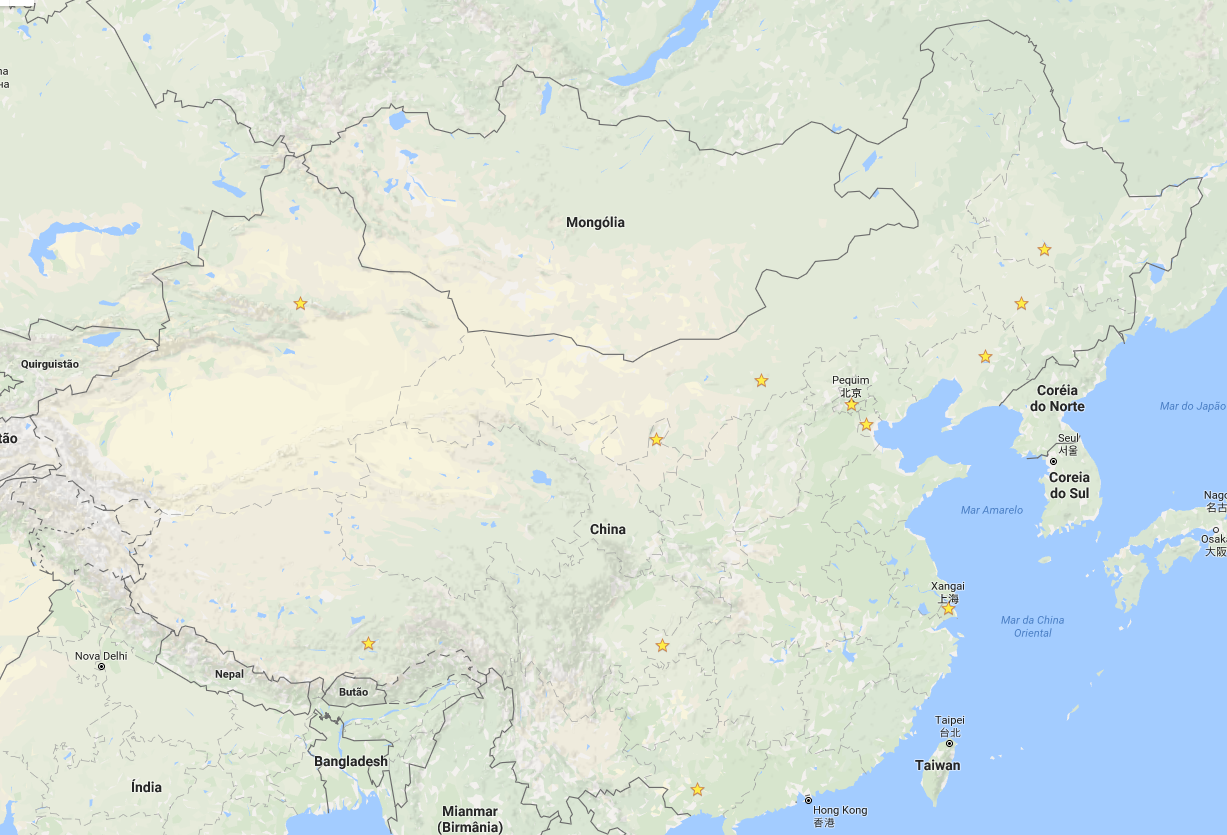
\includegraphics[width=0.55\columnwidth]{China_cities.png}
    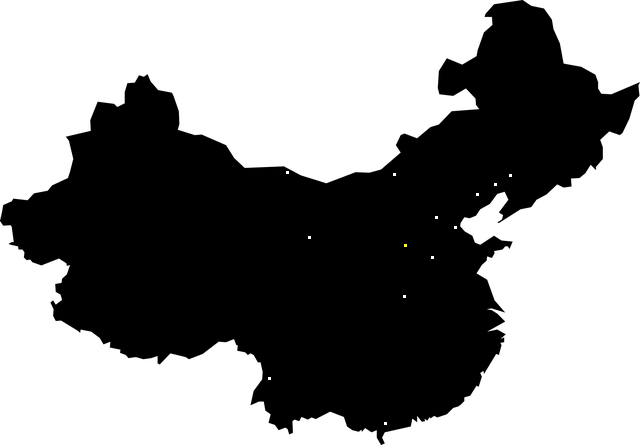
\includegraphics[width=0.5\columnwidth]{China_drawn.png}
    \caption{Comparação entre o mapa da China e o resultado obtido a partir do algoritmo desenvolvido no exerc\'icio 3.30b.}
  \end{figure}
\end{frame}

\begin{frame}
  \maketitle
\end{frame}

\end{document}